\begin{figure}
  \centering
    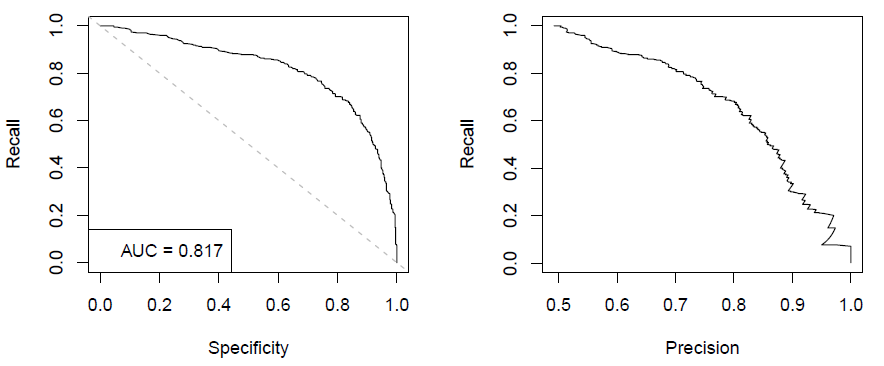
\includegraphics[width=0.5\textwidth]{media/bluecluster.png}
    \caption{Performances of CLEVER while cold-starting the last project in the blue cluster\label{fig:bluecluster}}
\end{figure}

\begin{figure}
  \centering
    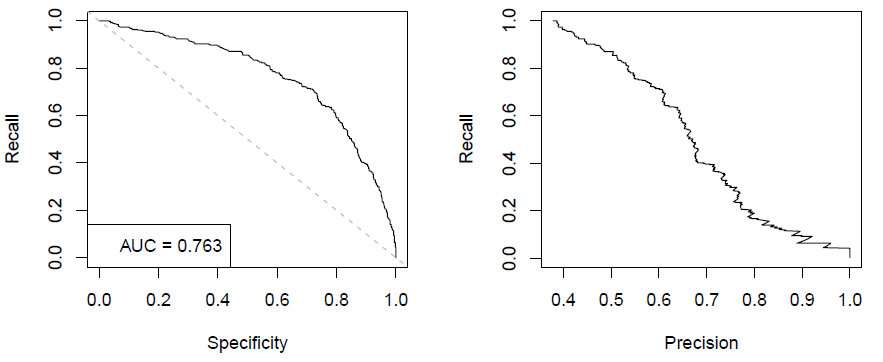
\includegraphics[width=0.5\textwidth]{media/yellowcluster.png}
    \caption{Performances of CLEVER while cold-starting the last project in the yellow cluster\label{fig:yellowcluster}}
\end{figure}


\begin{figure}
  \centering
    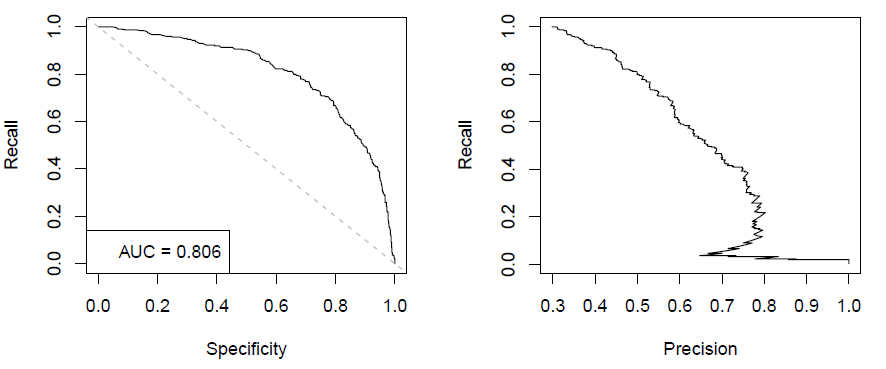
\includegraphics[width=0.5\textwidth]{media/redcluster.png}
    \caption{Performances of CLEVER while cold-starting the last project in the red cluster\label{fig:redcluster}}
\end{figure}

\begin{figure}
  \centering
    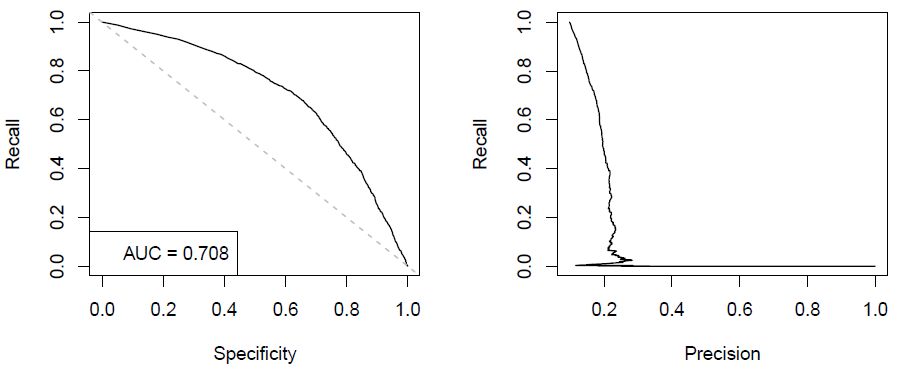
\includegraphics[width=0.5\textwidth]{media/redonblue.png}
    \caption{Performances of CLEVER while cold-starting the last project in the blue cluster with model built with data from the red cluster\label{fig:redonblue}}
\end{figure}